\subsection{Test setup}

Our program was written in C/C++ and compiled with Clang. All memory allocations were cache line boundary aligned. For parallelization we used C++11 cross-platform library \texttt{<thread>}.

All benchmarks were performed on a Linux desktop which has 16 GB ram and a Core i7 3770 CPU with the following specification:

\begin{itemize}
\item 4 * 3.4 GHz (Turbo Boost up to 3.9 GHz)
\item 4 * 32 KB L1 instruction cache
\item 4 * 32 KB L1 data cache (write back)
\item 4 * 256 KB L2 cache (write back)
\item Hyper-Threading
\item Shared 8 MB L3 cache (inclusive, write back)
\item 64 byte cache lines
\item The associativity for the cache levels are 8, 8 and 16 respectively
% http://www.ni.com/white-paper/11266/en#toc5
\end{itemize}

L2 cache faults and L3 cache faults were measured using Intel Performance Monitor Counter while branch mispredictions were measured using PAPI.

All tests were performed 5 times and the median was selected. The data in the matrices were randomly generated double precision floating points with
an uniform distribution. The range of the data was -1 to
1.

\subsection{Simple multiplication}

\subsubsection{Row-based layout}
Figure~\ref{fig:rnrnrn0} shows the measured running time and cache
faults encountered when running the naive matrix multiplier on
matrices with row layout.
\begin{figure}[h!]
  \centering
  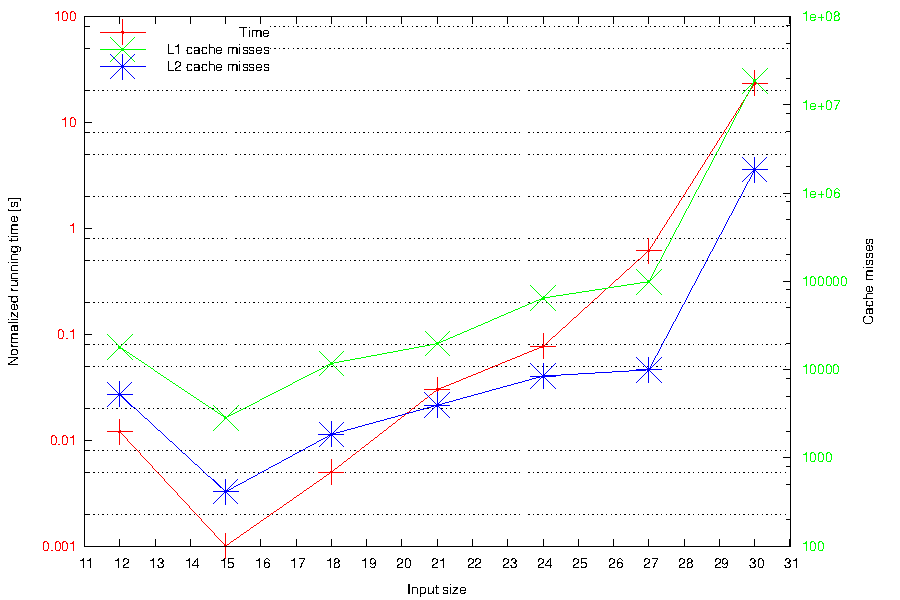
\includegraphics[width=\textwidth]{rnrnrn0.pdf}
  \caption{Running time and cache faults of naive matrix
    multiplication with all matrices using row layout.}
  \label{fig:rnrnrn0}
\end{figure}

As it can be seen in the plot, we start out by approximately the
expected number of L2 and L3 cache faults. However, the number of L2
cache faults quickly explodes, and the number of L3 cache faults also
far exceeds out expectations. It seems like the L2 cache begins to
perform very badly between instances of size $2^7 = 128$ and $2^8 =
256$, and that the L3 cache loose its performance when going from
$2^{9} = 512$ to $2^{10} = 1024$.

We highly suspect that the cache layout due to the 8-way associativity
is to blame. When looking up in the L2 cache, the 36 bit physical
address of the i7 processor is split into three parts $addr =
(tag,index,offset)$. Since the cache line size is $64b$, $6$ bits
should be used to reference a byte in a cache line. Because the L2
cache is $256kb$, we find that the index size to be
\[
  \frac{256 \cdot 1024}{\underbrace{64}_{\text{Cache line size}} \cdot \underbrace{8}_{\text{Cache associativity}}}
    = 512 = 2^9.
\]
Hence, we should use $9$ bits to specify the index. The remaining
$36-6-9=21$ bits is used as tag. Notice that the tag is the most
significant part of the address.

Because our matrices are square matrices of size a power of two, it
will always be the case that a new row in a matrix starts with a new
cache line. But this means that a cache line, and the corresponding
cache lines on the next row, always will be $\frac{n}{B}$ cache lines
apart. Therefore, when we read a matrix with row layout in a column
like fashion, we can only use $\frac{2^9}{\frac{n}{B}} =
\frac{2^9B}{n}$ cache lines. Since the L2 cache i 8-way associative,
we have to write to each entry before we begin to trash the cache
lines. Therefore we find that
\[
\frac{2^9 B}{n} \cdot \overbrace{8}^{\mathclap{\text{8-way associativity}}} \leq n
\iff
181 \approx \sqrt{2^9 \cdot 8^2} \leq n.
\]
When we exceed this number we should switch to our bad-case analysis
from the algorithms section. This switch occurs a lot earlier than
expected (the expected was $n$ around $2000$), because of the way the
cache is structured. Observe that this analysis predicts that we will
begin to trash the L2 cache between $n = 128$ and $n = 256$. This is
exactly what is measured in our experiments.

A similar analysis can be made for the L3 cache. It is a $16$-way
cache having $8$ megabytes of storage. This gives an index size of
$2^{13}$. Therefore we find that
\[
\frac{2^{13} \cdot B}{n} \cdot 16 \leq n \iff 1024 = \sqrt{2^{13} \cdot 8 \cdot 16} \leq n
\]
This is also where our experiments shows that the L3 cache begins to
trash it's values.

Figure~\ref{fig:rowrowfixed} shows a plot with the updated
expectations. It can be seen that these fits quiet good with our
measurements.
\begin{figure}[h!]
  \centering
  \missingfigure{Cache faults on naive row-row layout with updated expectations.}
  \caption{Cache faults on naive row-row layout with updated
    expectations.}
  \label{fig:rowrowfixed}
\end{figure}

\subsubsection{Combined row-based and column-based layout}

\ref{fig:rncnrn0}

\begin{figure}[h!]
  \centering
  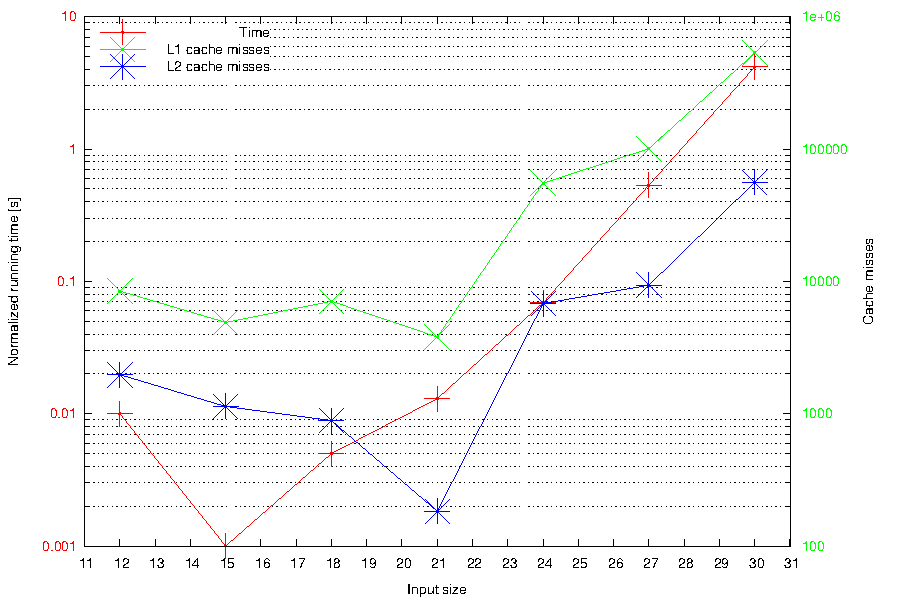
\includegraphics[width=\textwidth]{rncnrn0.pdf}
  \label{fig:rncnrn0}
\end{figure}

\subsection{Recursive multiplication}

\subsubsection{Z-curve layout}

\ref{fig:zrzrzr0}

\begin{figure}[h!]
  \centering
  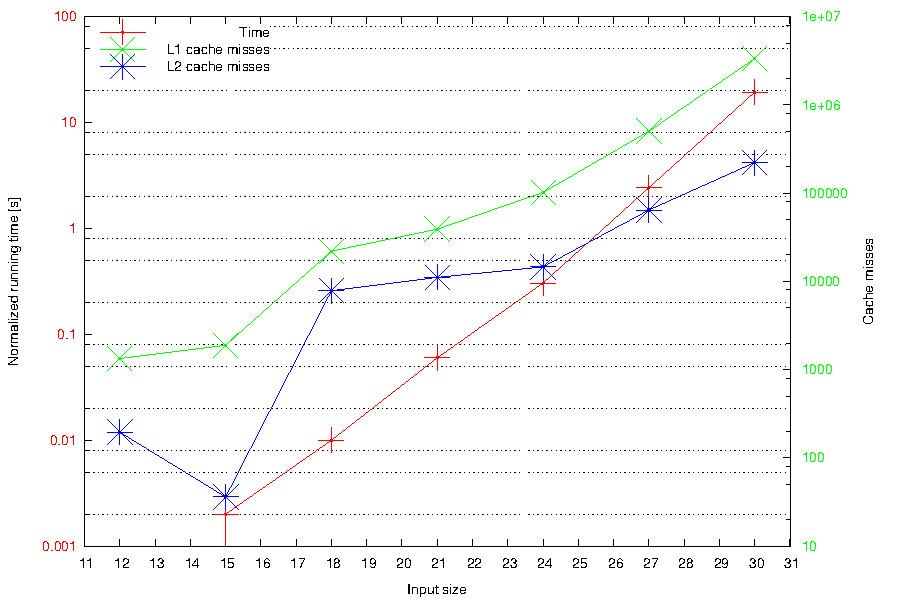
\includegraphics[width=\textwidth]{zrzrzr0.pdf}
  \label{fig:zrzrzr0}
\end{figure}

\subsection{Tiled layout}

\subsection{Strassen}

\todo{lig de 2 plots sammen, inkluder antal instruktioner og sig at det ikke er som forventet mht. cache faults}

\begin{figure}[h!]
  \centering
  \includegraphics[width=\textwidth]{"../project2/plots/4096/row-tiled8x8 recursive-8(tiled-bc)_column-tiled-8x8 recursive-8(generic-bc)_row-tiled8x8 recursive-8(tiled-bc)_0"}
  \caption{Recursive}
\end{figure}



\begin{figure}[h!]
  \centering
  \includegraphics[width=\textwidth]{"../project2/plots/4096/z-curve-tiled strassen-32(32-fixed-tiled-bc)_z-curve-tiled strassen-32(32-fixed-tiled-bc)_z-curve-tiled strassen-32(32-fixed-tiled-bc)_0"}
  \caption{Strassen}
\end{figure}